% First, tell LaTeX what kind of document you want to create. The most commonly-used is ``article'': it's sort of a catch-all generic class.
\documentclass[12pt]{article}  
% other built-in classes include report, book, beamer (slides), etc. Often, journals will have you use classes they created.

% % PREAMBLE: Define parameters for your document to use that don't get printed in the document. Here's where you include packages, style parameters, write your title, etc.

\title{Getting Started with \LaTeX: \\ 
	\large{A Biostatistics Brown Bag Seminar}}
\author{Nick Seewald}
\date{6 November 2015}

\usepackage{amsmath, amsfonts, amssymb, graphicx, float, lipsum, hyperref}
\usepackage[margin=1in]{geometry}


% To start making your document, open a ``document'' environment and start writing between the \begin{} and \end{} declarations

\begin{document}
	\maketitle
	
	\section{What is This?}
	
	Here are some terminological fun facts that go over great at parties.
	\begin{itemize}
		\item ``TeX'' is a markup language (like HTML) invented by Donald Knuth.
		\item A lot of hullabaloo has been made over the pronunciation of ``TeX''. From Knuth's \textit{TeXbook}:
		\begin{quote}
			Insiders pronounce the X of TeX as a Greek chi, not as an ‘x’, so that TeX rhymes with the word blecchhh. It’s the ‘ch’ sound in Scottish words like loch or German words like ach; it’s a Spanish ‘j’ and a Russian ‘kh’. When you say it correctly to your computer, the terminal may become slightly moist.
		\end{quote}
		My thoughts? Who cares. Just don't say ``tecks.'' It makes you seem like you don't know what you're doing.
		\item \LaTeX \ is more or less an offshoot of standard TeX that builds in a lot of nice features that make life easier.
	\end{itemize}
	
	\section{Installation}
	
	\begin{enumerate}
		\item The first thing you need is a \LaTeX \ \textit{distribution}. If you know Python, this is kind of analogous to Anaconda, Canopy, etc.
		\begin{itemize}
			\item \textit{If you use Windows:} download MiKTeX from \url{miktex.org}.
			\item \textit{If you use a Mac:} download MacTeX from \url{https://tug.org/mactex/}.
			\item \textit{If you use Linux:} download TeX Live from \url{https://www.tug.org/texlive/}. (TeX Live is also available for Mac and Windows, but behaves slightly differently than MiK/MacTeX)
		\end{itemize}
		\item You can write TeX in any standard text editor. In fact, a dedicated TeX editor usually comes with your \LaTeX \ distribution. But we're better than that.
		
		I like to use a cross-platform editor called \textit{TeXstudio}. Get it at \url{http://texstudio.sourceforge.net/}.
		
		For more (including some really nitty-gritty details), see \url{https://en.wikibooks.org/wiki/LaTeX/Installation}) \cite{wikibooks}
	\end{enumerate}
	
	
	\section{Basic Syntax}
	
	In a traditional word processor, what you see is what you get. With \LaTeX, however, you have to tell the program what you \textit{mean}. As a consequence, it comes with a bit of a learning curve, but once you get the hang of it, you can easily produce beautiful documents with rich math formatting and much more.
	
	\subsection{Commands}
	
	\LaTeX is built on \textit{commands}. A command can do a number of things. It can describe formatting instructions, or include a character or symbol that's not on your keyboard (like epsilon, $\epsilon$.) Commands start with \textbackslash and are followed by some text. You can provide input to commands by putting it in between braces, \textbraceleft \textbraceright. Let's look at some examples.
	
	\begin{table}[H]
		\centering
		\begin{tabular}{c|c}
			\textbf{\LaTeX Command} & \textbf{Result} \\ \hline
			\verb|\textit{Make text Italic}| & \textit{Make text Italic} \\
			\verb|\section{}| & Make a new section \\
			\verb|$\sqrt{4} = 2$| & $\sqrt{4} = 2$ \\ 
			\verb|$\bar{X}| & $\bar{X}$
		\end{tabular}
	\end{table}
	
	You'll notice that some of those commands are between \$'s. This is to indicate \textit{math mode}. The majority of commands in \LaTeX are meant to be used in math mode, which tells the compiler to making spacing, etc. behave nicely. Let's see an example.
	
	\begin{verbatim}
		\begin{quote}
		    To find estimates for $\alpha$ and $\beta$ in simple linear regression, 
		    we have to minimize the \textit{least-squares equation},
	    	\[
	            L(\alpha, \beta) = \sum_{i=1}^{n} \left(Y_{i} - \alpha - 
	            \beta X_{i}\right).
		    \]
		\end{quote}
	\end{verbatim}
	
	\begin{quote}
		To find estimates for $\alpha$ and $\beta$ in simple linear regression, we have to minimize the \textit{least-squares equation},
		\[
			L(\alpha, \beta) = \sum_{i=1}^{n} \left(Y_{i} - \alpha - \beta X_{i}\right).
		\]
	\end{quote}
	
	Notice that \verb|\alpha| and \verb|\beta| must be called in math mode. We can create ``displayed'' math (that appears on its own line) by surrounding the math with brackets: \verb|\[ \]|. We don't need to include \$'s here; the brackets indicate math mode for us. 
	
	If you get stuck and don't know the command to produce a particular symbol, try using DeTeXify: \url{detexify.kirelabs.org}.
	
	\subsection{Environments}
	
	An \textit{environment} behaves like a command, but applies its formatting rules to a larger part of the document. Open an environment using \verb|\begin{environmentname}| and close it using \verb|\end{environmentname}|. Options for how the environment works/looks can be provided in brackets following the \verb|\begin| statement. Here's an example of the \texttt{figure} environment:
	
	\begin{verbatim}
\begin{figure}[h]
    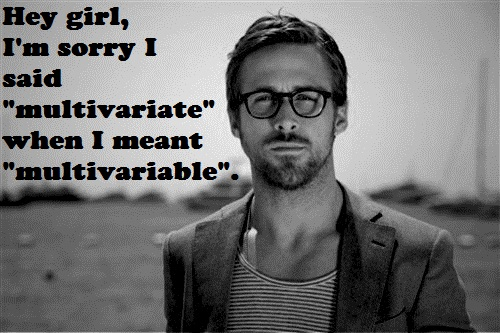
\includegraphics[width=.4\textwidth]{biostatryan.jpg}
    \caption{I forgive you, Ryan.}
    \label{fig: ryan gosling}
\end{figure}
	\end{verbatim}
	
	\begin{figure}[h]
		\centering
		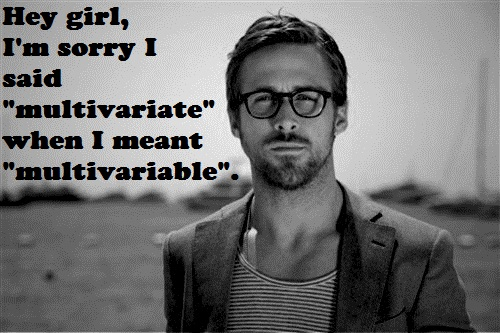
\includegraphics[width=.5\textwidth]{biostatryan.jpg}
		\caption{I forgive you, Ryan.}
		\label{fig: ryan gosling}
	\end{figure}
	
	There are a few key components included in the code to include Figure~\ref{fig: ryan gosling}. First is the \verb|[h]| option. \texttt{h} stands for \texttt{here}, which tells \LaTeX to put the figure approximately where the code is on the page. It won't always do that, though, because \LaTeX can (and will!) make decisions about where to put stuff to make things as pretty as it can. You can override this by using the \texttt{float} package, and specifying the \verb|[H]| option (which I think means \texttt{HERE!}).
	
	\begin{thebibliography}{99}
		\bibitem{wikibooks} ``LaTeX." Wikibooks, The Free Textbook Project. 23 Jan 2015, 02:30 UTC. 5 Nov 2015, 23:10 \url{https://en.wikibooks.org/w/index.php?title=LaTeX&oldid=2757849}.
	\end{thebibliography}
	
\end{document}